%----------------------------------------------------------------------------------------
%    PACKAGES AND THEMES
%----------------------------------------------------------------------------------------

\documentclass[aspectratio=169,xcolor=dvipsnames]{beamer}
\usetheme{SimpleDarkBlue}
\usepackage{subcaption}
\usepackage{amsmath, amsfonts, amssymb}
\usepackage[style=apa, backend=biber]{biblatex}
\addbibresource{references.bib}

\usepackage{hyperref}
\usepackage{graphicx} % Allows including images
\usepackage{booktabs} % Allows the use of \toprule, \midrule and \bottomrule in tables

%----------------------------------------------------------------------------------------
%    TITLE PAGE
%----------------------------------------------------------------------------------------

\title{Reflection \& Coxeter Groups}

\author{Shubkarman Walia}

\date{\today} % Date, can be changed to a custom date

%----------------------------------------------------------------------------------------
%    PRESENTATION SLIDES
%----------------------------------------------------------------------------------------

\begin{document}

\begin{frame}
    % Print the title page as the first slide
    \titlepage
\end{frame}

\begin{frame}{Overview}
    % Throughout your presentation, if you choose to use \section{} and \subsection{} commands, these will automatically be printed on this slide as an overview of your presentation
    \tableofcontents
\end{frame}

%------------------------------------------------
\section{Mirrors and Reflections}
%------------------------------------------------

\begin{frame}{Hyperplanes and Mirrors}
    \begin{block}{Hyperplane}
        In an $n$-dimensional vector space, an $n-1$ dimensional subspace is called a \alert{hyperplane}.
    \end{block}

    \begin{figure}
    \centering

    \begin{subfigure}[t]{0.3\textwidth}
        \centering
        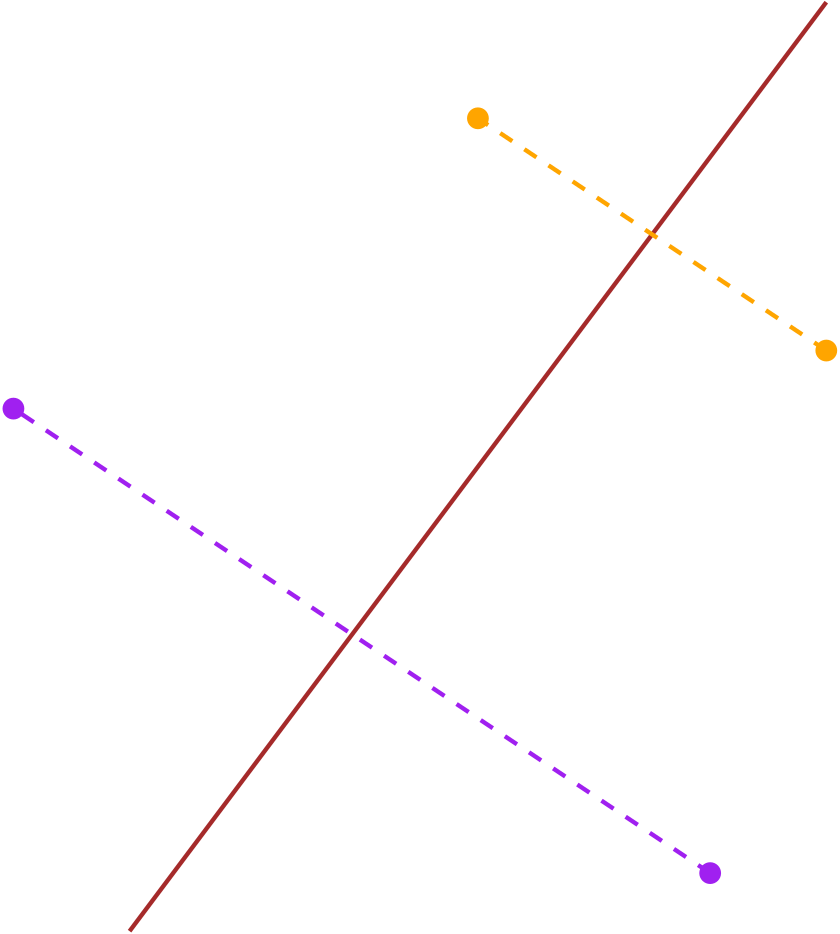
\includegraphics[width=0.9\linewidth]{2dMirror.png}
        \caption{Mirror in $\mathbb{R}^2$}
        \label{fig:subim1}
    \end{subfigure}
    \hspace{0.3cm}
    \begin{subfigure}[t]{0.3\textwidth}
        \centering
        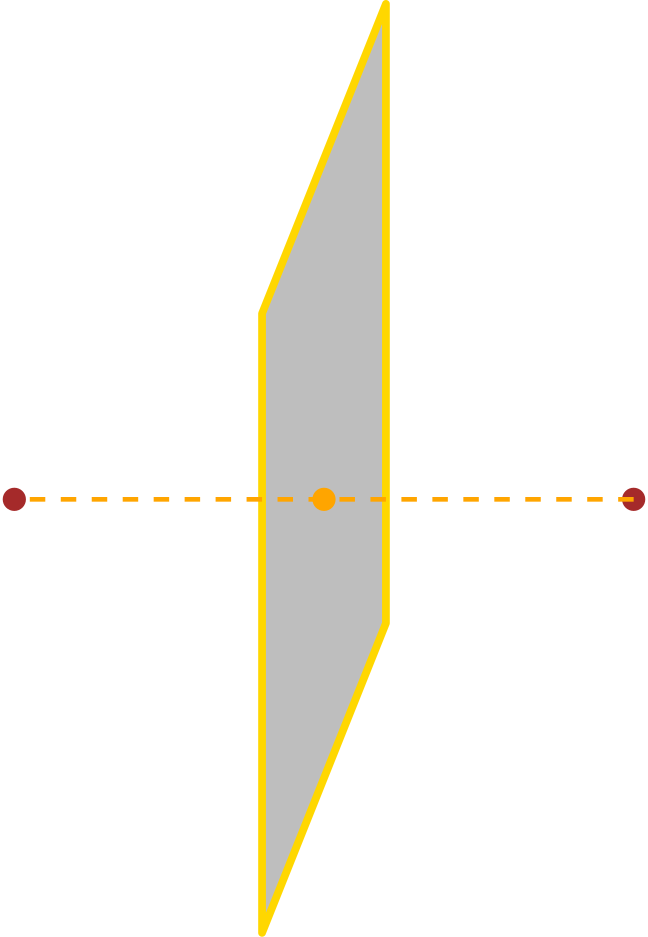
\includegraphics[width=0.9\linewidth]{mirror1.png}
        \caption{Mirror in $\mathbb{R}^3$}
        \label{fig:subim2}
    \end{subfigure}
    \hspace{0.3cm}
    \begin{subfigure}[t]{0.3\textwidth}
        \centering
        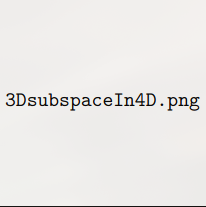
\includegraphics[width=0.9\linewidth]{3DsubspaceIn4D.png}
        \caption{Mirror in $\mathbb{R}^4$}
        \label{fig:subim3}
    \end{subfigure}
\begin{figure}
    \centering
    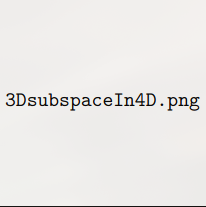
\includegraphics[width=0.5\linewidth]{3DsubspaceIn4D.png}
    \caption{Enter Caption}
    \label{fig:enter-label}
\end{figure}
    \label{fig:image2}
    \end{figure}

\end{frame}


%------------------------------------------------

\begin{frame}{A precise definition}
    

    \begin{block}{Reflections in a Vector space}
    Reflections are \alert{orthogonal transformations}. Hence they preserve distance and angles. 

    So if $s$ is a reflection and $\alpha, \beta \in \mathbb{R}^n$ then, $||s(\alpha)||= ||\alpha||$ and $s(\alpha). s(\beta)=\alpha.\beta$
    \end{block}

    \begin{alertblock}{More Precisely}
        Reflection in a Real Euclidean Vector space endowed with a positive definite symmetric bilinear form $(\lambda , \mu)$ is a linear operator that sends some non-zero vector $\alpha$ (normal to the hyperplane $H_{\alpha})$ to its negative while fixing everything in the hyperplane $H_{\alpha}$.
    \end{alertblock}
\end{frame}

%------------------------------------------------

\begin{frame}{Reflection as an orthogonal transformation}
    \begin{block}{Fact}
        The set of all orthogonal transformations of a vector space $V$ forms a group, $O(V)$.
    \end{block}
    And so, a \alert{finite} group generated by a system of mirrors (multiple reflections) is just a subgroup of O(V).
\end{frame}

%------------------------------------------------


\begin{frame}{Some Examples}
    \begin{figure}
        \centering
        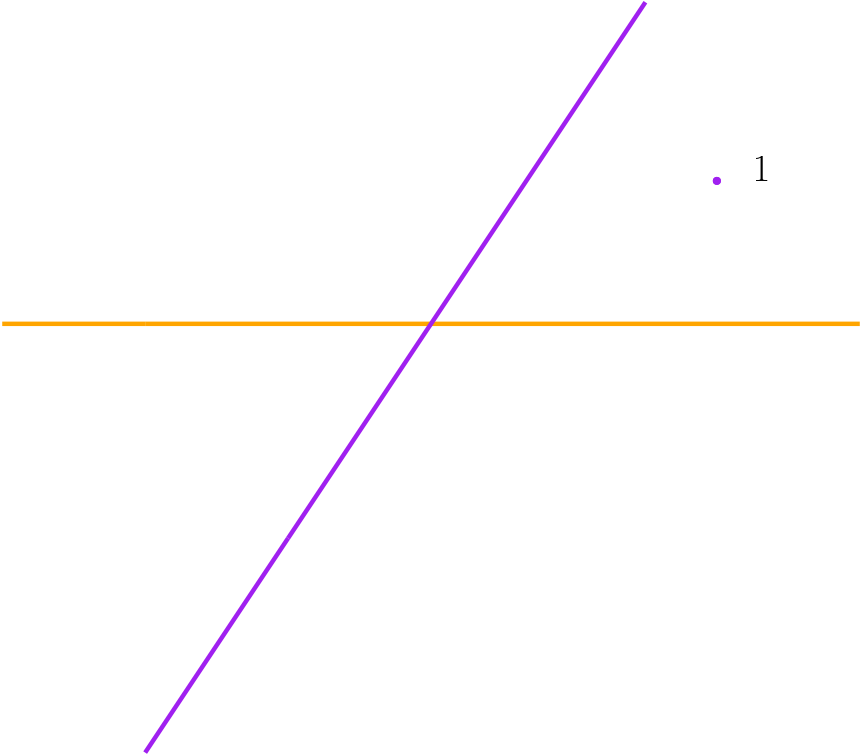
\includegraphics[width=0.5\linewidth]{frameN-6.png}
        \label{fig:enter-label}
    \end{figure}
\end{frame}

%------------------------------------------------

\begin{frame}{Some Examples}
    \begin{figure}
        \centering
        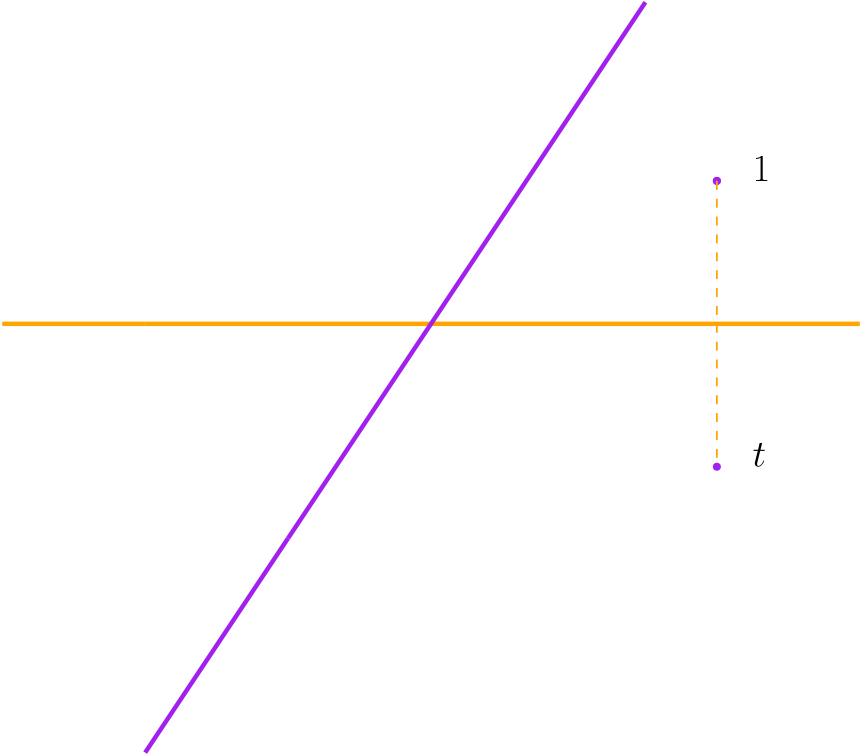
\includegraphics[width=0.5\linewidth]{frameN-5.png}
        \label{fig:enter-label}
    \end{figure}
\end{frame}
%------------------------------------------------

\begin{frame}{Some Examples}
    \begin{figure}
        \centering
        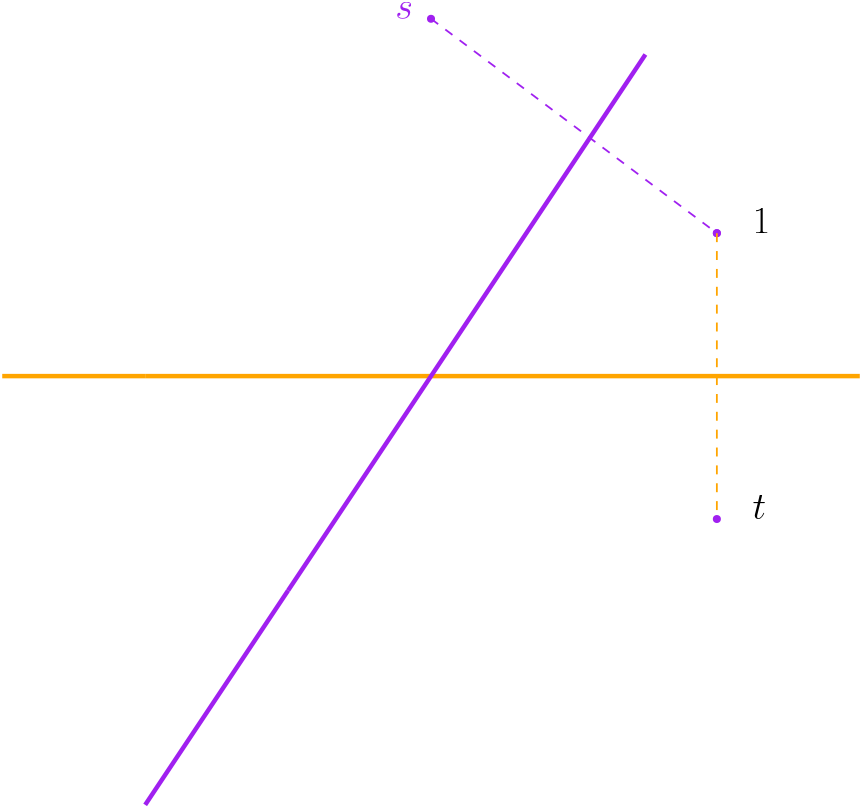
\includegraphics[width=0.5\linewidth]{frameN-4.png}
        \label{fig:enter-label}
    \end{figure}
\end{frame}
%------------------------------------------------

\begin{frame}{Some Examples}
    \begin{figure}
        \centering
        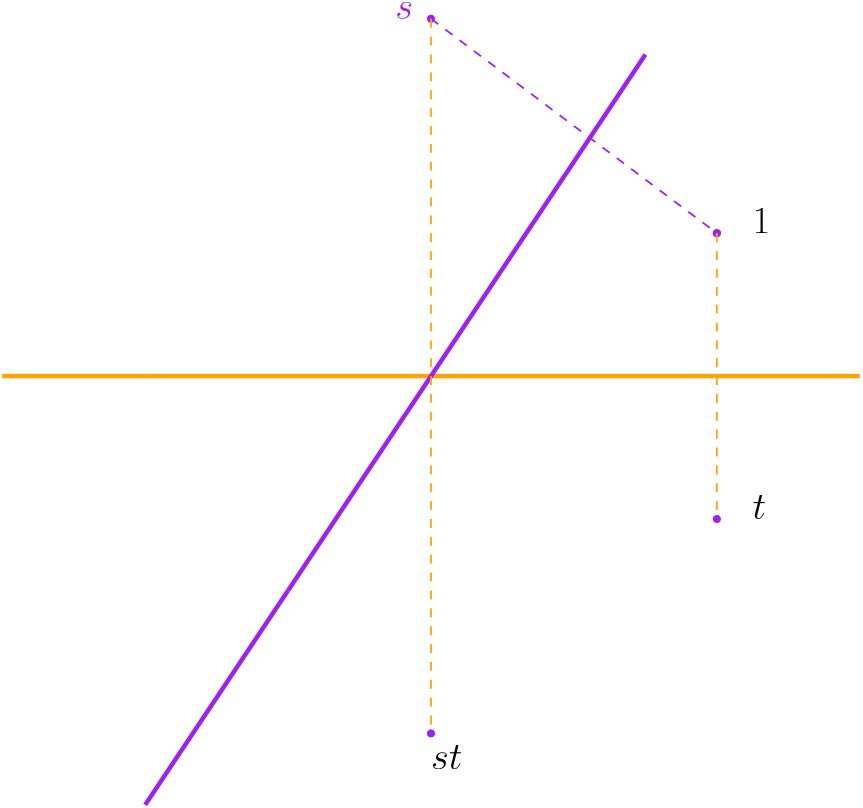
\includegraphics[width=0.5\linewidth]{frameN-3.png}
        \label{fig:enter-label}
    \end{figure}
\end{frame}
%------------------------------------------------

\begin{frame}{Some Examples}
\begin{figure}
    \centering
    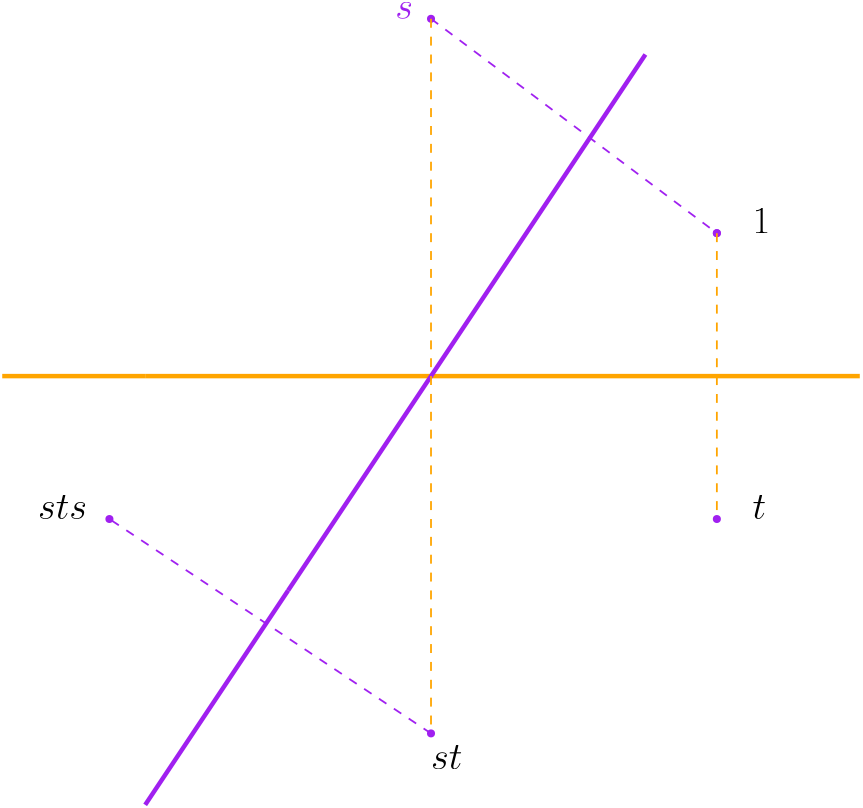
\includegraphics[width=0.5\linewidth]{frameN-2.png}
    \label{fig:enter-label}
\end{figure}
\end{frame}
%------------------------------------------------

\begin{frame}{Some Examples}
    \begin{figure}
        \centering
        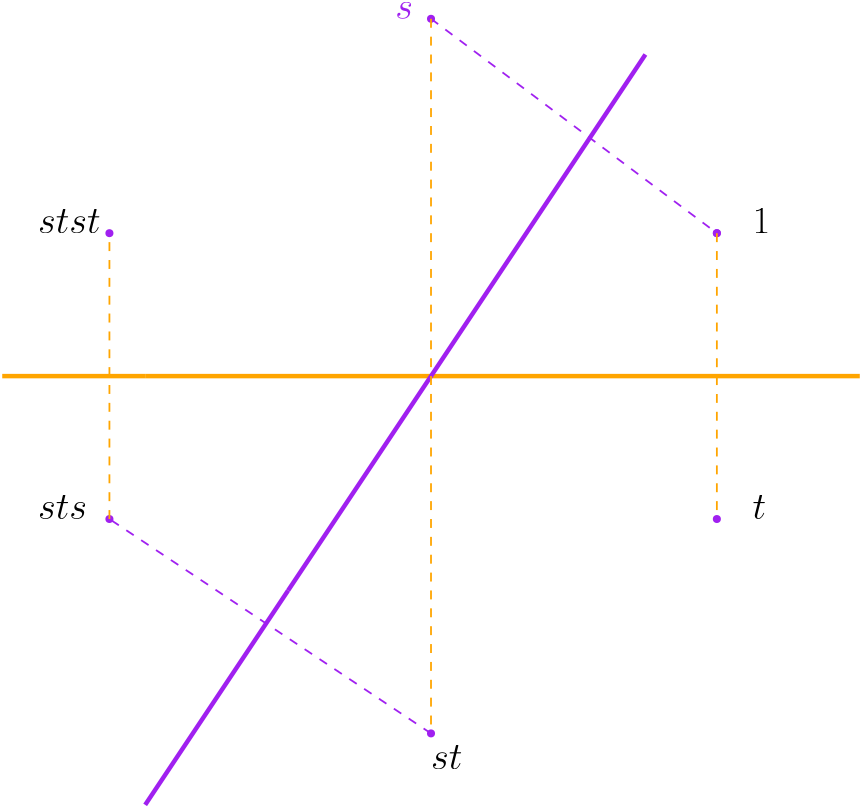
\includegraphics[width=0.5\linewidth]{frameN-1.png}
        \label{fig:enter-label}
    \end{figure}
\end{frame}

\begin{frame}{Some Examples}
    \begin{figure}
        \centering
        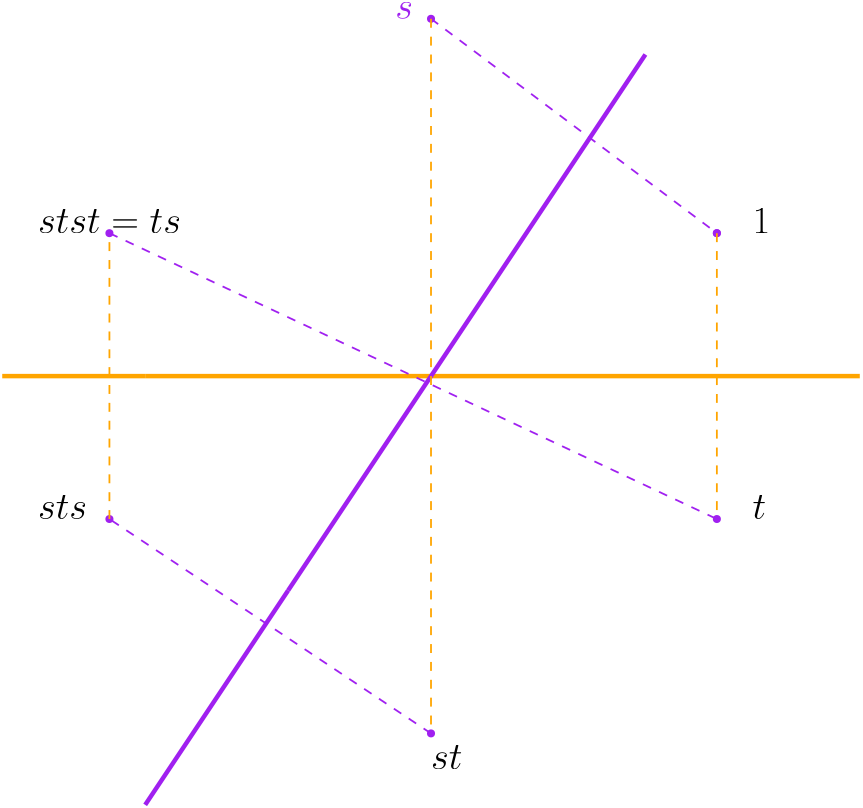
\includegraphics[width=0.5\linewidth]{frameN.png}
        \label{fig:enter-label}
    \end{figure}
    
\end{frame}
%------------------------------------------------
\begin{frame}{Some Examples}
    \begin{columns}
    
        \begin{column}{0.5\textwidth}
            \centering
            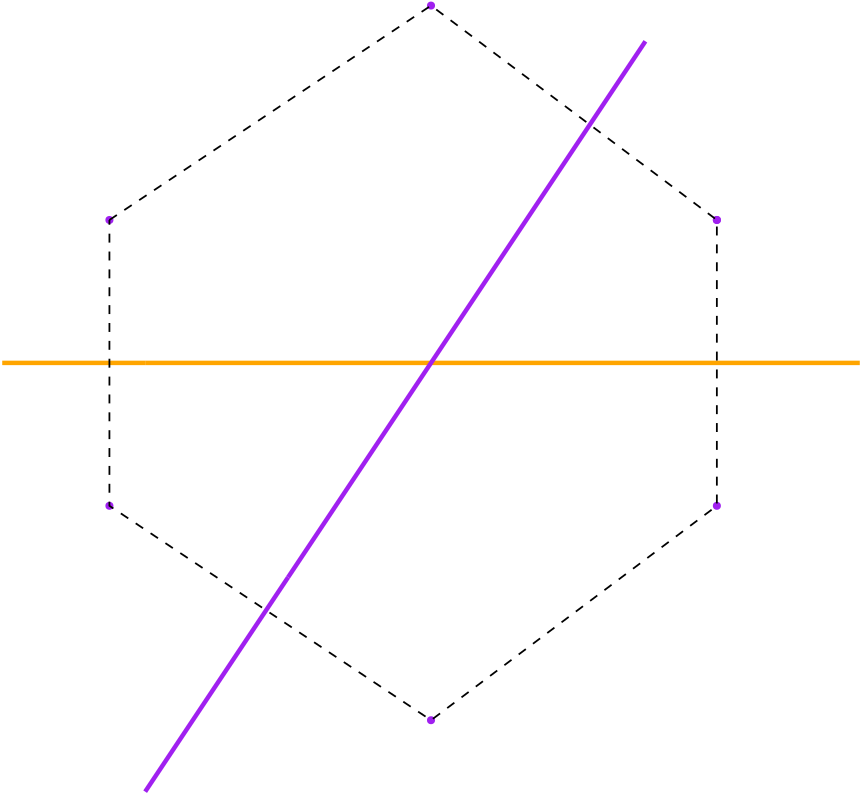
\includegraphics[width=0.9\linewidth]{frameLast.png}
        \end{column}

        \begin{column}{0.5\textwidth}
            \begin{block}{Conclusion}
                \begin{itemize}
                    \item $s^2 = t^2 = 1$ for any reflection $s, t$
                    \item We get only 6 (finite) number of "images" or elements of the group.
                    \item We get this mysterious relation: $sts = tst$
                    \item We get the group: 
                        $\langle s, t \mid s^2 = t^2 = 1,\ sts = tst \rangle$

                \end{itemize}
            \end{block}
        \end{column}

    \end{columns}
\end{frame}


%------------------------------------------------

\begin{frame}{Another Example}
\begin{figure}
    \centering
    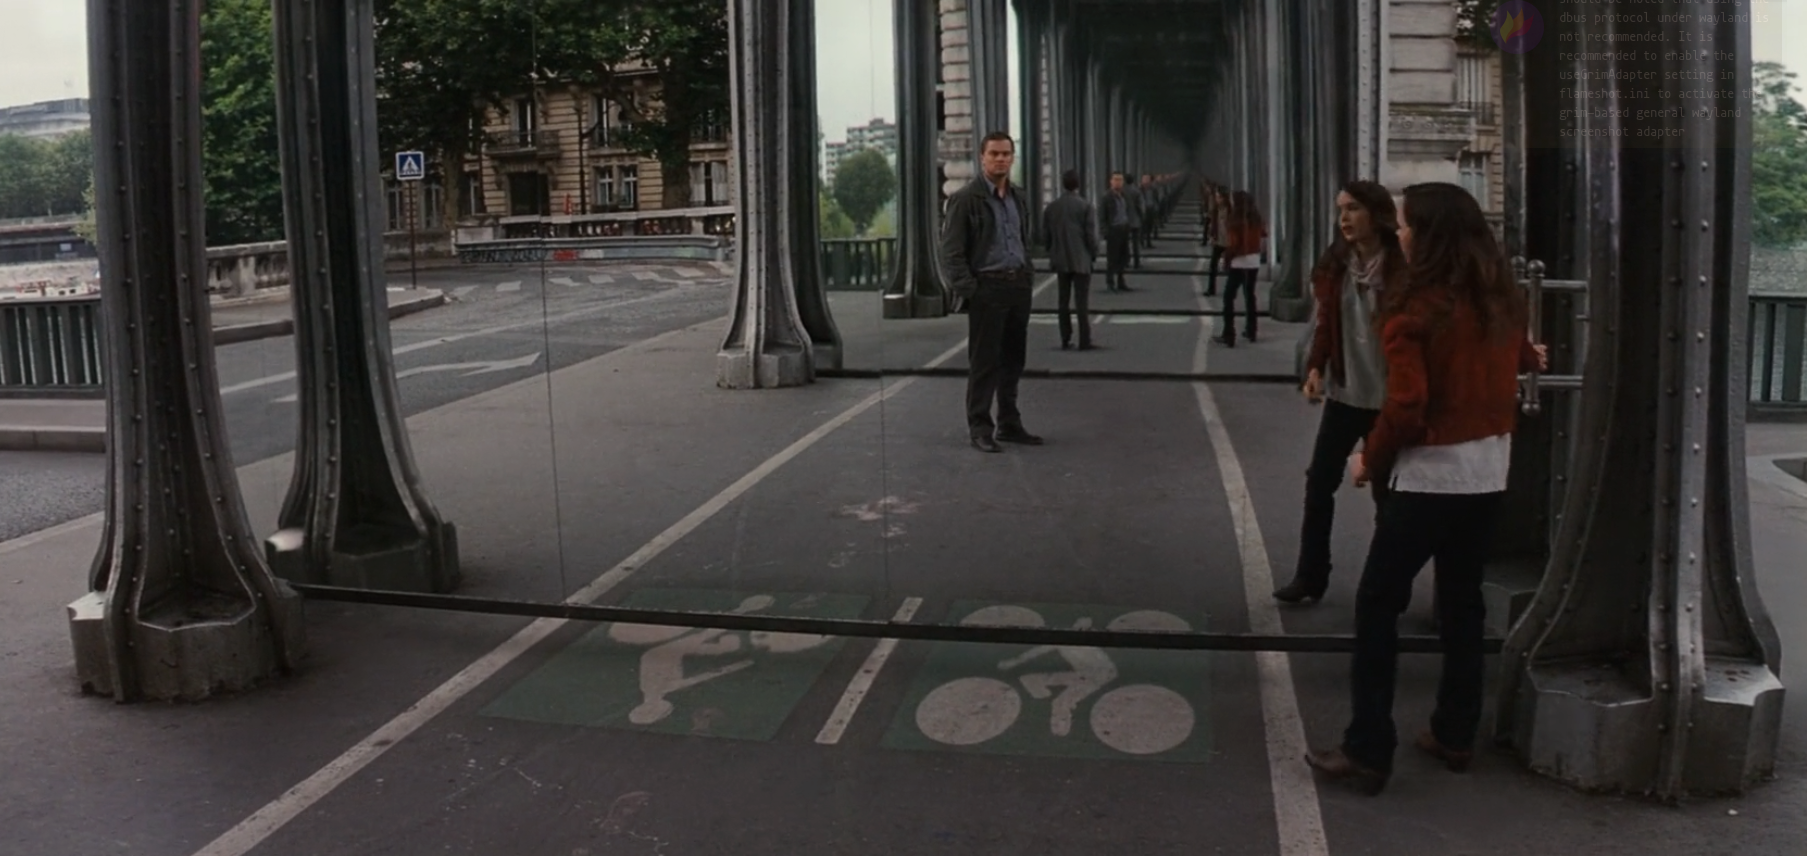
\includegraphics[width=1\linewidth]{inceptionMirror.png}
    \caption{$\tilde{A_2}$ in Inception}
    \label{fig:enter-label}
\end{figure}
\end{frame}

\begin{frame}{Another Example}
    \begin{figure}
        \centering
        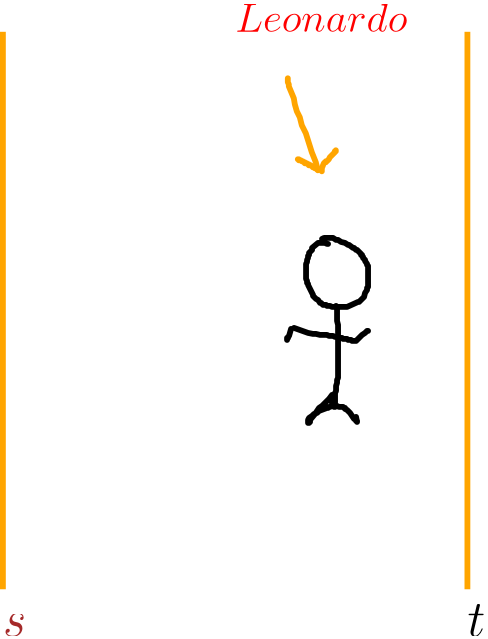
\includegraphics[width=0.35\linewidth]{leonardo.png}
        \caption{Inception Sketch}
        \label{fig:enter-label}
    \end{figure}

\end{frame}

\section{Coxeter Groups}

%------------------------------------------------

\begin{frame}{How to find all the Finite Configurations?}
    \begin{theorem}
        The group of all isometries of $\mathbb{AR}^n$ which fix a point $o$ coincides with the orthogonal group $\mathbb{O}_n$.
    \end{theorem}
    \begin{alertblock}{Consequence}
        The finite groups generated by reflections, i.e, Finite Reflection Groups,
        fix a point.
    \end{alertblock}
    And so, all the hyperplanes in a system of mirrors must have a point in common in order to generate finite images.
\end{frame}

%------------------------------------------------
\begin{frame}{Enter: Coxeter Systems}
    \begin{block}{Coxeter system}
        A Coxeter system is a group generated by a finite set of generators 
        \[S = \{s_1, s_2, ... , s_n\} \]
        under the relations: 
        \[s_i^2=1 \text{ for all }1\leq i \leq n\]

        \[\underbrace{s_i s_j s_i \cdots}_{m_{ij}\ \text{terms}}=\underbrace{s_i s_j s_i \cdots}_{m_{ij}\ \text{terms}}\text{ for all } 1 \leq i, j \leq n\]
    \end{block}
    
\end{frame}

\begin{frame}{An Example}
    \[S=\{s, t\} \text{ with } m_{st}=3\]
    \[\implies W = \langle s, t| s^2=t^2=1, sts=tst\rangle \]
\end{frame}


\begin{frame}{An Example}

    \setlength{\columnsep}{0.1em}

    \begin{columns}
        \begin{column}{0.5\textwidth}
            And we know $W = $
        \end{column}

        \begin{column}{0.5\textwidth}
            \centering
            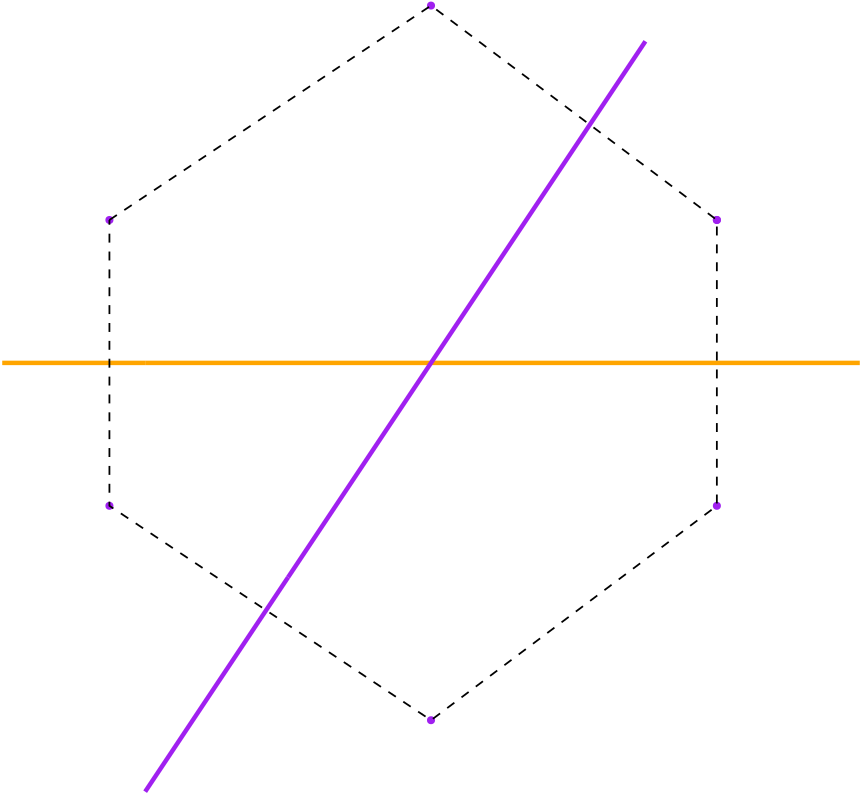
\includegraphics[width=0.9\linewidth]{frameLast.png}
        \end{column}
    \end{columns}

\end{frame}

\begin{frame}{Equivalence}
\begin{alertblock}{The Connection}
    Each finite reflection group can be represented as a coxeter system.
\end{alertblock}
And so we have turned a geometrical problem to a combinatorial one!    
\end{frame}

\begin{frame}{Coxeter Graphs}
    \begin{block}{Representation of Coxeter systems}
        Each Coxeter system can be represented as a graph where each vertex is a generator of the corresponding Coxeter group, and there's an edge between vertices if $m_{ij}\geq3$ with edge label$=m_{ij}$.
    \end{block}
\end{frame}

\begin{frame}{A combinatorial approach}
We saw before how $\langle s, t\rangle$ with $m_{st} =3$ was the finite group $D_6$

What about? 
\begin{figure}
    \centering
    \includegraphics[width=0.5\linewidth]{A{21}.png}
    \caption{Enter Caption}
    \label{fig:enter-label}
\end{figure}
\end{frame}

\begin{frame}{Frame Title}
    Notice, $(abc)^n \in W $ $\forall n\in \mathbb{N}$
    The group generated is infinite!
\end{frame}

\begin{frame}{A more elegant way}
Let $S=\{s_1, s_2, ..., s_n\}$ be the generator set of our Coxeter system.
Encode the Coxeter graph into a Coxeter matrix, say A, known as the \alert{Cartan Matrix} such that 

\[(a_{ij}) = (a_{ji})= -cos(\pi/m_{ij}) \text{ for } s_i, s_j \in S\]

\begin{alertblock}{Note}
    A is a symmetric matrix so all of its eigenvalues $\in \mathbb{R}$
\end{alertblock}

\begin{theorem}
    If A is positive definite, i.e all eigenvalues of A are strictly positive then the Coxeter system associated to A is finite.\\
    If A is positive semi-definite, i.e all eigenvalues of A are non-negative (zeroes are allowed) then the associated Coxeter System is affine.
\end{theorem}
    
\end{frame}


\begin{frame}{Computing}
    All that remains is to see all possible Coxeter systems that are possible and compute its eigenvalues...
    \begin{figure}
        \centering
        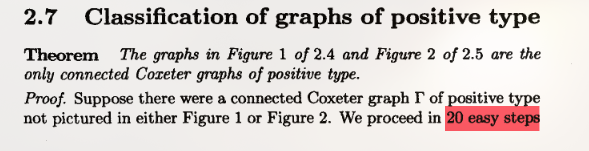
\includegraphics[width=0.5\linewidth]{HumphreysTheorem1.png}
        \caption{Humphreys: pg 36}
        \label{fig:enter-label}
    \end{figure}
\end{frame}

\begin{frame}{20 Easy Steps}
   \begin{figure}
       \centering
       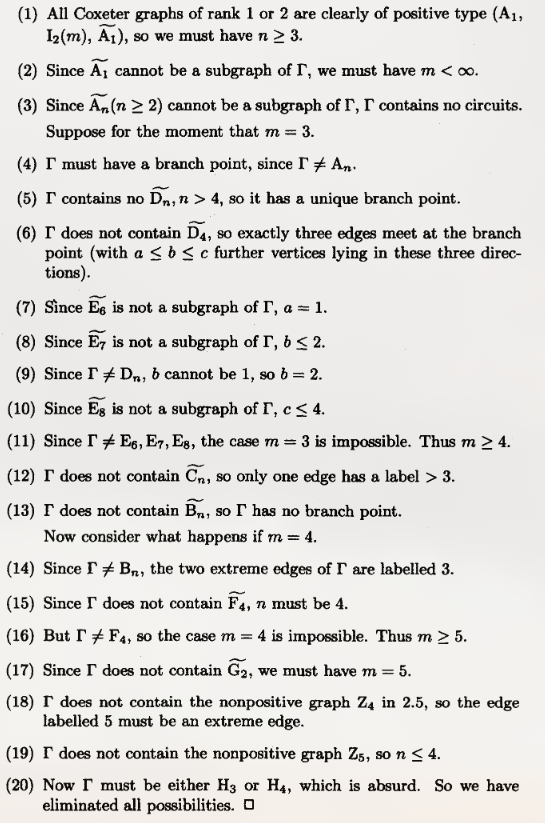
\includegraphics[width=0.32\linewidth]{20EasySteps.png}
       \caption{Humphreys: 20 Easy steps}
       \label{fig:enter-label}
   \end{figure}
\end{frame}

\begin{frame}{Finite Classification}
    \begin{figure}
        \centering
        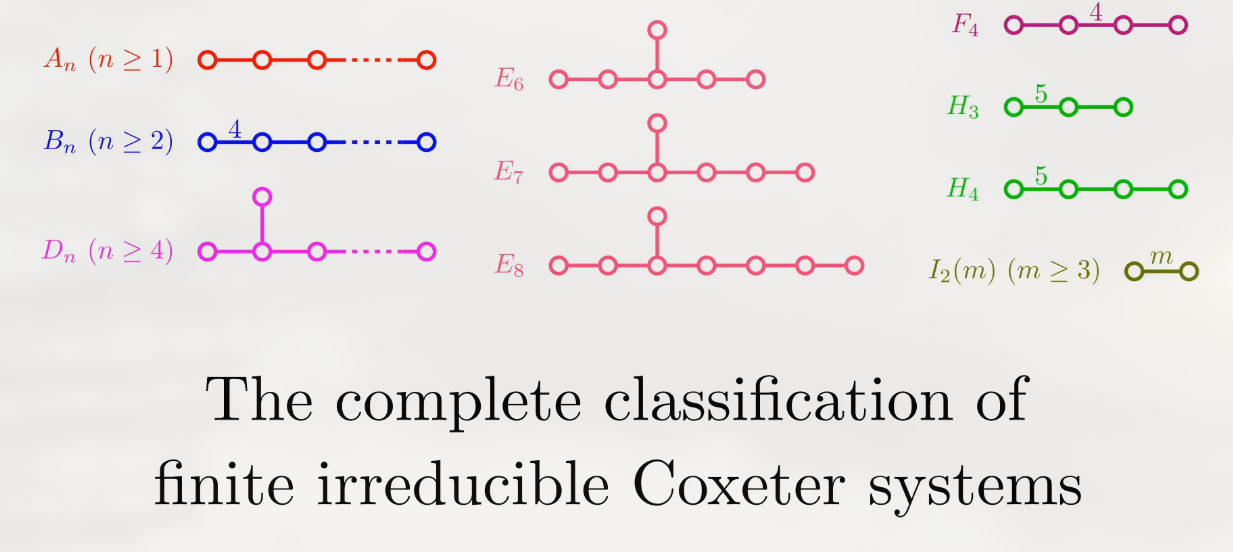
\includegraphics[width=1\linewidth]{FiniteClassification.png}
        \caption{All possible ways you can orient mirrors in n-dimensions so that you get finite images.\\Credits for the Image: Joseph Newton}
        \label{fig:enter-label}
    \end{figure}
\end{frame}


\begin{frame}{References}
\begin{itemize}
    \item Alexandre V. Borovik, \& Anna Borovik. (2010). \textit{Mirrors and Reflections: The Geometry of Finite Reflection Groups}. Springer.
    \item James E. Humphreys. (1990). \textit{Reflection Groups and Coxeter Groups}. Cambridge University Press.
    \item Newton, J. [Joseph Newton]. (n.d.). \textit{The Coxeter Classification} [Video]. YouTube. \url{https://www.youtube.com/watch?v=BV5mYjh8m4E&t=402s}
\end{itemize}

\end{frame}




%------------------------------------------------

\begin{frame}
    \Huge{\centerline{\textbf{Thank you!}}}
\end{frame}

%----------------------------------------------------------------------------------------

\end{document}